\documentclass{article}
\usepackage[ascii]{inputenc}
\usepackage{amsmath}
\usepackage{amssymb,amsfonts,textcomp}
\usepackage[T1]{fontenc}
\usepackage[english]{babel}
\usepackage{color}
\usepackage{array}
\usepackage{hhline}
\usepackage{hyperref}
\usepackage{algorithm}
\usepackage{algpseudocode}

\hypersetup{pdftex, colorlinks=true, linkcolor=blue, citecolor=blue, filecolor=blue, urlcolor=blue, pdftitle=, pdfauthor=kenlo dinh-van, pdfsubject=, pdfkeywords=}
\usepackage[pdftex]{graphicx}
\providecommand\textsubscript[1]{\ensuremath{{}_{\text{#1}}}}
% Text styles
\newcommand\textstyleHeadingiiiChar[1]{\textrm{\textcolor[rgb]{0.12156863,0.21568628,0.3882353}{#1}}}
% Outline numbering
\setcounter{secnumdepth}{0}
% Footnote rule
\setlength{\skip\footins}{0.119cm}
\renewcommand\footnoterule{\vspace*{-0.018cm}\setlength\leftskip{0pt}\setlength\rightskip{0pt plus 1fil}\noindent{\rule{0.25\columnwidth}{0.018cm}}\vspace*{0.101cm}}
% Pages styles
\makeatletter
\newcommand\ps@Standard{
  \renewcommand\@oddhead{}
  \renewcommand\@evenhead{}
  \renewcommand\@oddfoot{}
  \renewcommand\@evenfoot{}
  \renewcommand\thepage{\arabic{page}}
}
\makeatother
\pagestyle{Standard}

\title{SOEN 6011: Project Team C Student N4}
\author{Kenlo DINH VAN (26641652)}
\date{}

\begin{document}
\maketitle

\section[1 Function Description]{{1 Function Description}}}
\subsection[1.1 Logarithmic Function]{\textbf{{1.1 Logarithmic Function}}}
\begin{equation*}
\log _b(x)
\end{equation*}
The \textbf{{logarithmic}} function is the \textbf{{inverse}} of the exponential function, since it is a one-to-one function.
The graph of an inverse function is the reflection of the original function, using the line y = x as reflection axis.
John Napier expressed y as a function of x for the logarithm in 1614 resulting in:

\begin{equation*}
\log _b(x)=y
\end{equation*}
{which can be read: ``x is equal to b (base) to the power y'', which is equivalent to {\textquotedbl}y
is the base-b logarithm of x.{\textquotedbl}}

{\centering  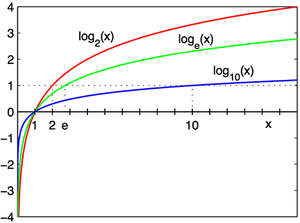
\includegraphics[width=5.44cm,height=4.038cm]{N4PB12-img001.png} \par}


 \begin{description}
  \item[$\bullet$] \textbf{{Domain}{:}}{ x {\textgreater} 0
(set of positive real numbers) }
  \item[$\bullet$] \textbf{{Co-domain}}{: Set of real numbers
}\textbf{{R}}
\item[$\bullet$]{\textbf{{Specificity of the base}}}{: b ${\neq}$ 1 and b
{\textgreater} 0}
\end{description}



\subsection[1.2 Unique characteristics]{\textbf{{1.2 Unique characteristics}}}
{Exponential expressions can be written as logarithmic expressions and logarithmic expressions can be
written as exponential expressions. ex: 3}{\textsuperscript{2}}{=9 ={\textgreater}
log}{\textsubscript{3}}{(9) = 2}

\liststyleWWNumiithm }

		  \itemsmize}
          
          
          \begin{description}
  \item[$\bullet$] when b = 10 the function is called common logarithm and is denoted log(x)
  \item[$\bullet$] when b = }\textit{{e}} = 2.718... function is called natural logarithm and denoted ln(x)
\end{description}

\subsubsection[Change of base ]{\textbf{{Change of base }}}
{\displaystyle \log _{b}x={\frac {\log _{k}x}{\log _{k}b}}.\,}
\subsubsection[Logarithmic identities ]{\textbf{{Logarithmic identities}}}

   \begin{description}
  \item[$\bullet$] {Product: } $\log _b(x\ast y)=\log _bx+\log _by$
 \item[$\bullet$]  {Quotient: } $\log _b(x/y)=\log _bx-\log _by$
 \item[$\bullet$]  {Power: } $\log _b(x^p)=p\log _bx$
 \item[$\bullet$] {Root: } $\log _b\sqrt[p]x=\frac{\log _bx} p$
\end{description}
%  \clearpage
\section[2. Assumptions]{\textbf{{2. Assumptions}}}
\subsubsection[Assumption 1 ]{\textbf{{Assumption 1 }}}
{As of version 0, we assume that the user interface will be text based relying on console
input-output.}

\subsubsection[Assumption 2 ]{\textbf{{Assumption 2 }}}
{The `system' refers to the scientific calculator, Eternity: Functions}

\section[3. Functional requirements]{\textbf{{3. Functional requirements}}}
\subsubsection[F4.0.v1 Function Selection ]{\textbf{{F4.0.v1 Function Selection }}}
{When the system starts, the interface should display the function name and allow the user to select
the logarithmic function.} \textbf{ Priority: Low, Risk: Low, Difficulty: Low}

\subsubsection[F4.1.v1 Logarithm Base Initialization ]{\textbf{{F4.1.v1 Logarithm Base Initialization
}}}
{When the user selects the logarithmic function, the system should ask the user which base
}\textit{{b}}{ he wishes to use and set the base value.}\textbf{ Priority: Medium, Risk: Low, Difficulty: Low}

\subsubsection[F4.2.v1 Logarithm Base Validation]{\textbf{{F4.2.v1 Logarithm Base Validation}}}
{After the user inputs the base value }\textit{{b}}{, the system
should validate that }\textit{{b}}{ is a real positive number not equal to 1.}\textbf{ Priority: Medium, Risk: Low, Difficulty: Medium}

\subsubsection[F4.3.v1 Logarithm Variable Initialization]{\textbf{{F4.3.v1 Logarithm Variable
{If the base }\textit{{b}}{ is valid, the system should ask the user
to input the value for variable }\textit{{x }}{and set it.} \textbf{ Priority: Medium, Risk: Low, Difficulty: Low}

\subsubsection[F4.4.v1 Logarithm Variable Validation]{\textbf{{F4.4.v1 Logarithm Variable Validation}}}
{After the user inputs the variable }\textit{{x}}{ value, the system
should validate that the variable }\textit{{x}}{ is a real positive number.}\textbf{ Priority: Medium, Risk: Low, Difficulty: Medium}

\subsubsection[F4.5.v1 Logarithm Calculation]{\textbf{{F4.5.v1 Logarithm Calculation}}}
{If the variable }\textit{{x}}{ is valid, the system should calculate
the logarithm of }\textit{{x}}{ in base
}\textit{{b,}}{ without relying on java built-in functions, and store the result.}\textbf{ Priority: High, Risk: High, Difficulty: High}

\subsubsection[F4.6.v1 Result Display]{{F4.6.v1 Result Display}}}
{After the calculation completes, the system should display the result on the user interface.}\textbf{ Priority: Low, Risk: Low, Difficulty: Low}

\section{4. Considered Algorithms}

\subsection{4.1 Algorithm 1: Binary Logarithm Approximation}

The binary logarithm may be computed in two parts: an integer part (characteristic) and a fractional part (mantissa of the logarithm). 

\begin{equation*}
\log _{2}x=n+\log _{2}y\quad {\text{where }}y=2^{-n}x{\text{ and }}y\in [1,2)
\end{equation*}
\begin{description}
  \item[$\bullet$] \textbf{{Advantages}{:}} Mathematically sound, potential for a very precise result due to this 2 parts binary log value approximation.
(set of positive real numbers) }
  \item[$\bullet$] \textbf{{Disadvantages}}{: Complex. For practicality, this infinite series must be truncated to reach an approximate result. 
\end{description}
\begin{algorithm} [H] 
\caption{Binary Logarithm Approximation}
\label{alg:myalgo}
\begin{algorithmic}[1]
\Function{Logarithm}{$x,  $ base} \funclabel{} \label{alg:a-line}
    \State $r\gets \Call{Binary Log}{$x$}  /  \Call{Binary Log}{$base$}$
    \State \Return $r$
\EndFunction
\Statex
\Function{Binary Log}{$x$} \funclabel{} 
    \State $n\gets \Call{Binary Log Integer}{$x$}$
    \State $y\gets x/ 2^n$
    \State $f\gets \Call{Binary Log Fraction}{$y$}$
    \State \Return $b\gets n + f$ \Comment{returns the integer and fractional parts}
\EndFunction
\Statex
\Function{Binary Log Integer}{$x$} \Comment{returns 'p' a power of 2}
\State $p\gets 0$
\State $v\gets 1$
\While{$v\leq x$}
\State $v\gets v*2$
\If {$v<$ $x$ }
            \State $p\gets p+1$
    \EndIf
\EndWhile\label{}
 \State \Return $p$
\EndFunction
\Statex
\Function{Binary Log Fraction}{$y$} \funclabel{}
\If {$y==$ $1$ }
            \State \Return $0$ 
    \EndIf
   \State $z\gets y$
\State $m\gets 0$
\While{$z< 2$} \Comment{square until z in [2;4)]}
\State $z\gets z^2$
 \State $m\gets m+1$
\EndWhile\label{}
 \State \Return $log_2y\gets 2^-^m + 2^-^m \Call{Binary Log Fraction}{\frac{z}{2}} $  
    
\EndFunction
\end{algorithmic}
\end{algorithm}
\clearpage
\subsection{4.2 Algorithm 2: Natural Algorithm Approximation}

The second algorithm will rely on approximating the natural logarithm by considering the following identity:

\begin{equation*}
\ln(x)\ =\ \lim_{n\rightarrow\infty}\ n{\ (\ x^{1/n}\ }-\ 1)}
\end{equation*}
\begin{description}
  \item[$\bullet$] \textbf{{Advantages}}{:} Simpler to implement.
  \item[$\bullet$] \textbf{{Disadvantages}}{:} Possible lack of precision.
\end{description}
\begin{algorithm}[H]
\caption{Natural Logarithm Approximation}
\label{alg:myalgo}
\begin{algorithmic}[1]
\Function{Logarithm}{$x,  $ base} \funclabel{} \label{alg:a-line}
    \State $r\gets \Call{Natural Log}{$x$}  /  \Call{Natural Log}{$base$}$
    \State \Return $r$
\EndFunction
\Statex
\Function{Natural Log}{$x$} \funclabel{}
  \State $a\gets 1000$
    \State \Return $n\times (x^(^1^/^n^) - 1)$
\EndFunction
\end{algorithmic}
\end{algorithm}

\section[References]{{References}}}
{[1] }\url{https://en.wikipedia.org/wiki/Logarithm}\\
{[2] }\url{https://en.wikipedia.org/wiki/Binary_logarithm}\\
{[3] }\url{http://dwb4.unl.edu/Chem/CHEM869R/CHEM869RMats/Logs/Logs.html}
\end{document}
